\documentclass[titlepage=firstiscover, captions=tableheading, bibliography=totoc]{scrartcl}
\usepackage[autostyle=true,german=quotes]{csquotes}
\usepackage{scrhack}
\usepackage{enumitem}
\usepackage{caption}
\usepackage[aux]{rerunfilecheck}
\usepackage{subcaption}
\usepackage{fontspec}
\usepackage[dvips]{graphicx}
\usepackage{floatflt,epsfig}

\usepackage{polyglossia}
\setmainlanguage{german}

\usepackage[unicode]{hyperref}
\usepackage{bookmark}
\title{Computational Physics}
\subtitle{Übungsblatt 7}
\author{
Miriam Simm\\
\texorpdfstring{\href{mailto:miriam.simm@tu-dortmund.de}{miriam.simm@tu-dortmund.de}\and}{,}
Katrin Bolsmann\\
\texorpdfstring{\href{mailto:katrin.bolsmann@tu-dortmund.de}{katrin.bolsmann@tu-dortmund.de}}{,}\\
\\
Mario Alex Hollberg\\
\texorpdfstring{\href{mailto:mario-alex.hollberg@tu-dortmund.de}{mario-alex.hollberg@tu-dortmund.de}}{}
}
\date{Abgabe: 15. Mai 2020}
\usepackage{amsmath}
\usepackage{amssymb}
\usepackage{mathtools}
\usepackage[
    math-style=ISO,
    bold-style=ISO,
    sans-style=italic,
    nabla=upright,
    partial=upright,
]{unicode-math}

\setmathfont{Latin Modern Math}

\usepackage[
  locale=DE,
  separate-uncertainty=true,
  per-mode=symbol-or-fraction,
]{siunitx}

\usepackage{multicol}
\setlength{\columnsep}{1pt} %space between columns

\usepackage{booktabs}
\usepackage[x11names, table]{xcolor}
\usepackage{graphicx}
\usepackage{grffile}
\usepackage{xfrac}
\usepackage{xcolor}

\usepackage{float}
\floatplacement{figure}{h}
\floatplacement{table}{h}
\usepackage[
  section,
  below,
]{placeins}

\usepackage{expl3}
\usepackage{xparse}
\ExplSyntaxOn
\NewDocumentCommand \E {} {\symup{e}}
\ExplSyntaxOff

% Literaturverzeichnis
\usepackage[
  backend=biber,
]{biblatex}
% Quellendatenbank
\addbibresource{literatur.bib}

\usepackage[
  version=4,
  math-greek=default,
  text-greek=default,
]{mhchem}


\raggedcolumns


\begin{document}

\maketitle

\section*{Aufgabe 1: Fouriertransformation}
Ziel der Aufgabe ist die Berechnung und Implementierung der schnellen Fouriertransformation (FFT). Die Fouriertransformation
ist hier definiert als
\begin{equation*}
	F \left(k\right) = \int_{-\infty}^{\infty} \, f(x) \, \text{e}^{ikx} \, \text{d}x
\end{equation*}
\begin{itemize}[leftmargin=*]
\item[1.] Zuerst wird die diskrete Fouriertransformation (DFT) als schnelle Fouriertransformation implementiert. Verwendet
					werden $N = 2^m$ Diskretisierungspunkte.
					\begin{equation*}
						F_j = \sum_{l=0}^{N-1} \Omega_N^{j,l} f_l
					\end{equation*}
					Zur Überprüng des Algrorithmus mit $m \in \left\{3, 4\right\}$ und
					\begin{equation*}
						f_l = \sqrt{(1+l)}
					\end{equation*}
					wird die Berechnung zusätzlich direkt implementiert. Bei beiden Werten von $m$ ergeben sich die gleichen
					Ergebnisse.
\item[2.] Der Ergebnisvektor $\vec{F}$ der in Teil 1 berechnet wird, muss noch verändert werden um die Ergebnisse der
					Fouriertransformation zu enthalten. Dazu werden die Elemente des Vektors verschoben und mit einem Phasenfaktor
					multipliziert
					\begin{equation*}
						F'_j = F_j \cdot \frac{\increment x}{2 \pi} \text{exp}\left(-2 \pi i x_\text{min} \frac{j}{L}\right)
					\end{equation*}
					Die Implementierung wird nun mit der Funktion
					\begin{equation*}
						f\left(x\right) = \text{e}^{-\frac{x^2}{2}}
					\end{equation*}
					auf dem Intervall $x \in \left[-10, 10\right]$ mit $m = 7$ getestet. Zum Vergleich wird zudem die analytische
					Lösung berechnet
					\begin{align*}
						\mathcal{F}\left[f\right](k)
											&= \frac{1}{2 \pi} \int_{-\infty}^{\infty}  \text{e}^{-\frac{x^2}{2}} \text{e}^{-i k x} \, \text{d}x \\
											&= \frac{1}{2 \pi} \int_{-\infty}^{\infty}  \text{e}^{-\frac{x^2}{2}-i k x} \, \text{d}x \\
											&= \frac{1}{2 \pi} \int_{-\infty}^{\infty}  \text{e}^{-\frac{1}{2}\left(x^2+2ik-k^2\right) - \frac{k^2}{2}} \, \text{d}x \\
											&= \frac{1}{2 \pi} \int_{-\infty}^{\infty}  \text{e}^{-\frac{1}{2}\left(x+ik\right)^2-\frac{k^2}{2}} \, \text{d}x \\
											&= \frac{\text{e}^{-\frac{k^2}{2}}}{\sqrt{2 \pi}} \, ,
					\end{align*}
					wozu im letzten Schritt das Gauß-Integral
					\begin{equation*}
						\int_{-\infty}^{\infty}  \text{e}^{-a\left(x+b\right)^2}  \, \text{d}x = \sqrt{\frac{\pi}{a}}
					\end{equation*}
					verwendet wurde.
					Zum besseren Vergleich sind die Ergebnisse außerdem in Abbildung \ref{fig:fig1} dargestellt. Man sieht deutlich,
					dass es sich bei der Fouriertransformierten der Gaußfunktion wieder um eine Gaußfunktion handelt, wie auch die
					analytische Lösung zeigt.
					\FloatBarrier
					\begin{figure}[H]
					    \centering
					    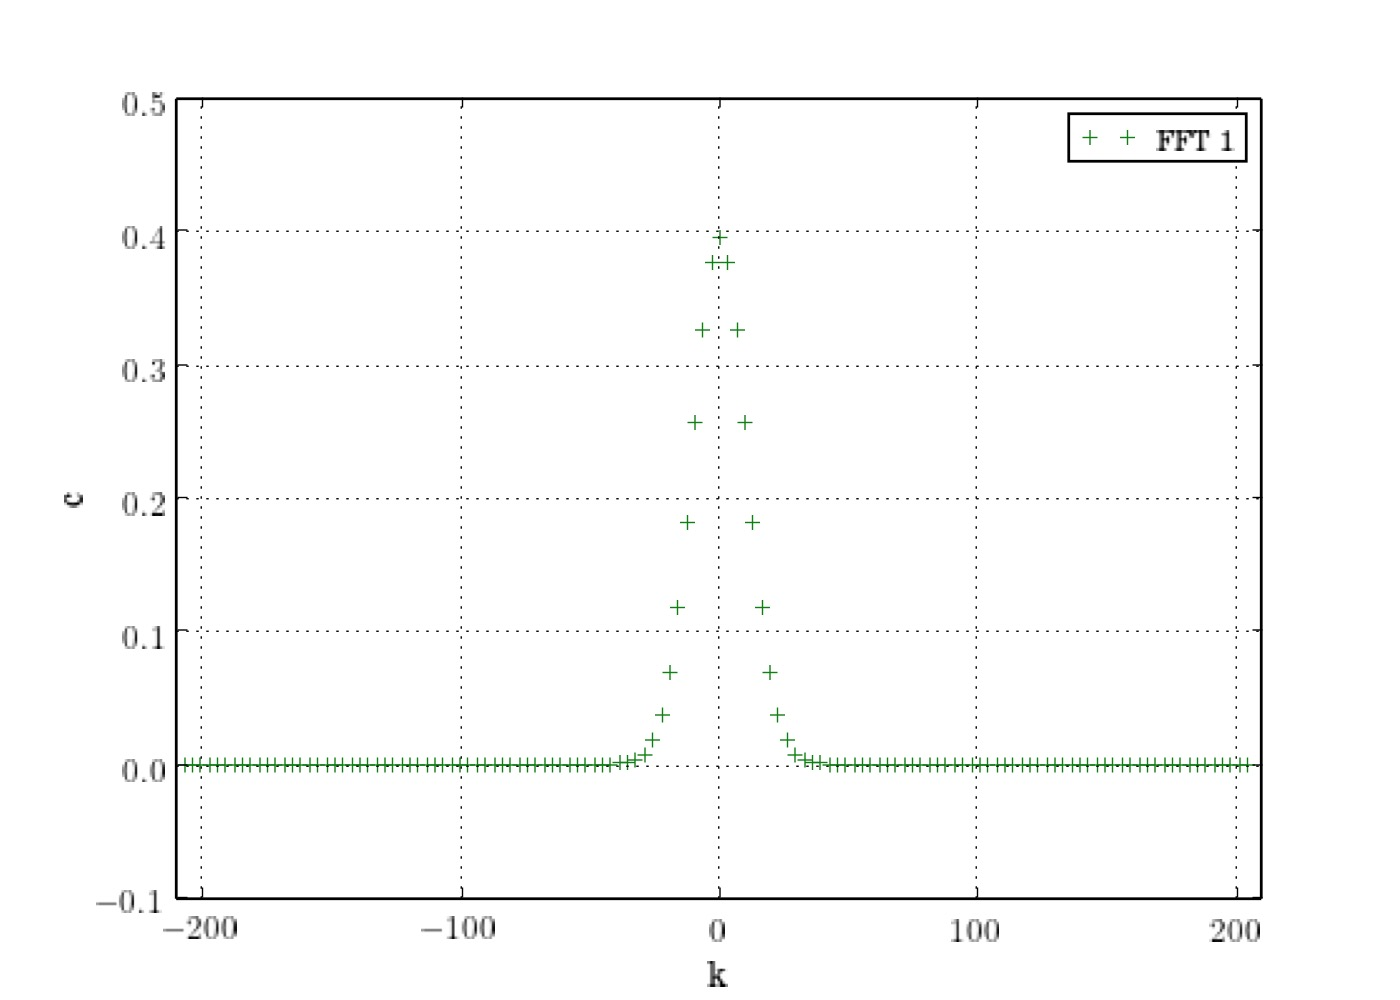
\includegraphics[width=0.8\textwidth]{a_1_1.jpg}
					    \caption{Fouriertransformierte der Gaußfunktion.}
					    \label{fig:fig1}
					\end{figure}
					\FloatBarrier
					\noindent
\item[3.] Die Implementierung wird nun zusätzlich mit der Rechteckschwingung verglichen
					\begin{equation*}
						f\left(x\right) = \begin{cases}
																-1, & x \in \left[-\pi, 0\right] \\
																1,  & x \in \left(0, \pi\right) \,
															\end{cases}
					\end{equation*}
					die $2 \pi$-periodisch ist. Die schelle Fouriertransformation wird nun verwendet, umd die komplexen Fourierkoeffizienten $c_k$ von $f(x)$ zu berechnen. In Abbildung \ref{fig:fig2} ist der Absolutbetrag der
					Koeffizienten grafisch dargestellt.
					\FloatBarrier
					\begin{figure}[H]
							\centering
							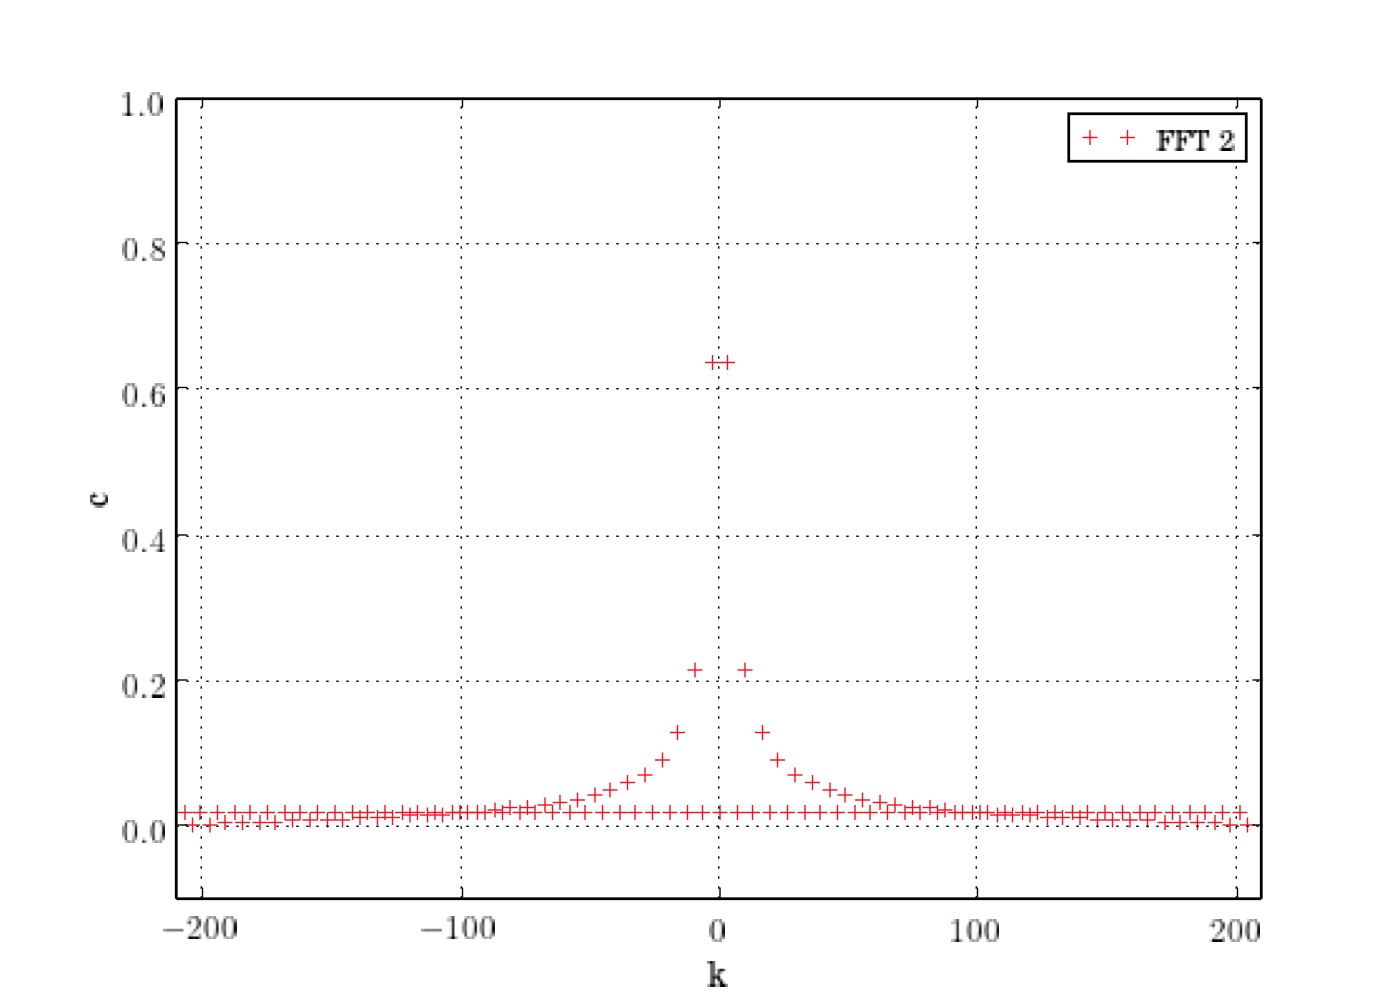
\includegraphics[width=0.8\textwidth]{a_1_2_1.jpg}
							\caption{Komplexe Fourierkoeffizienten der Rechteckschwingung, berechnet mit schneller Fouriertransformation.}
							\label{fig:fig2}
					\end{figure}
					\FloatBarrier
					\noindent
					Zum Vergleich der Ergebnisse wird außerdem die analytische Berechung durchgeführt
					\begin{align*}
						c_k &= \frac{1}{2 \pi} \int_{-\pi}^{\pi} \, f(x) \, \text{e}^{-ikx} \, \text{d}x \\
								&= \frac{1}{2 \pi} \int_{-\pi}^{0} \, -1 \, \text{e}^{-ikx} \, \text{d}x + \frac{1}{2 \pi} \int_{0}^{\pi} \, 1 \, \text{e}^{-ikx} \, \text{d}x \\
								&= \frac{1}{2 \pi}\left[\frac{1}{ik}  \text{e}^{-ikx}\right]_{-\pi}^0 + \frac{1}{2 \pi}\left[-\frac{1}{ik}  \text{e}^{-ikx}\right]_{0}^{-\pi} \\
								&= \frac{1}{2 \pi} \left(\frac{1}{ik}-\frac{1}{ik}\text{e}^{-ik\pi}-\frac{1}{ik}\text{e}^{ik\pi}+\frac{1}{ik}\right) \\
								&= \frac{i}{\pi k} \left(\cos(k\pi)-1\right) \\
								&= \begin{cases}
									-\frac{2i}{\pi k}, & k \, \text{ungerade} \\
									0,  & k \, \text{gerade} \,
							\end{cases}
					\end{align*}
					In Abbildung \ref{fig:fig3} ist der Verlauf der analytisch berechneten Kurve dargestellt. Auch hier zeigt sich, dass die Implementierung im Rahmen einer gewissen Ungenauigkeit korrekte Ergebnisse erzeugt, da beide Kurven den
					gleichen Verlauf haben.
					\FloatBarrier
					\begin{figure}[H]
							\centering
							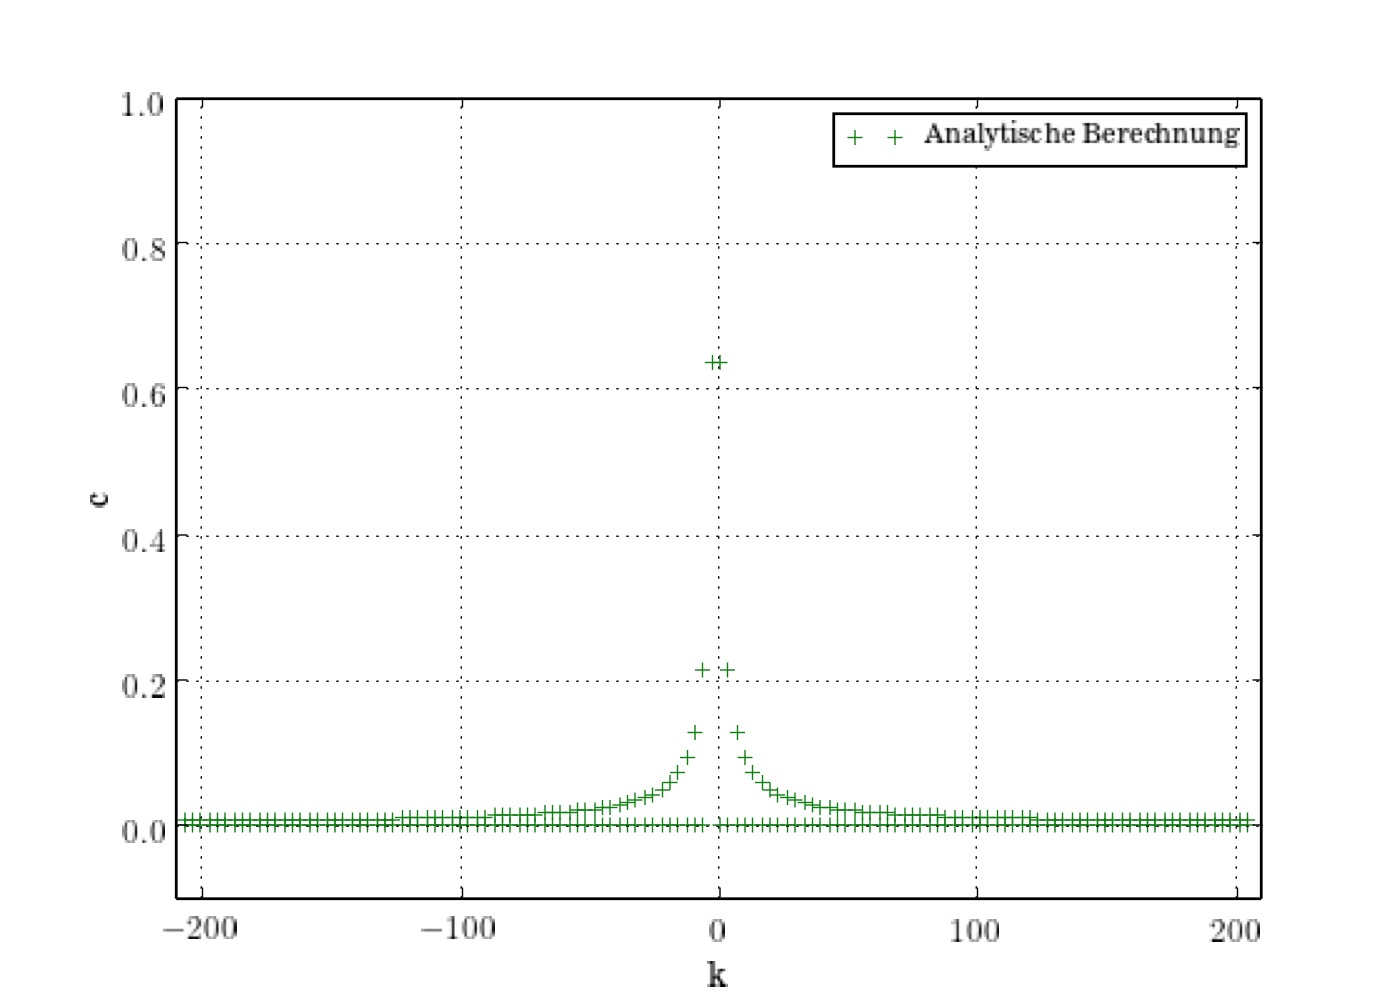
\includegraphics[width=0.8\textwidth]{a_1_2_2.jpg}
							\caption{Analytisch berechnete komplexe Fourierkoeffizienten der Rechteckschwingung.}
							\label{fig:fig3}
					\end{figure}
					\FloatBarrier
					\noindent
\end{itemize}

\section*{Aufgabe 2: Eindimensionale Minimierungsverfahren}

Mittels zweier unterschiedlicher Verfahren sollen das Minima der Funktion
\begin{equation*}
  f(x) = x^2 - 2
\end{equation*}

\noindent
gefunden werden. Die dabei benötigten Iterationsschritte werden in Tabelle
\ref{tab:A2} wiedergeben.

\begin{table}
\centering
\begin{tabular}{c c c}
  \toprule
  $\text{Verfahren}$          & $\text{Intervallhalbierung}$ & $\text{Newton}$  \\
  \midrule
  $\text{Iterationsschritte}$ & 61                           & 2                \\
  \bottomrule
\end{tabular}
\caption{Die Genauigkeitsschranke liegt bei $x_{\text{c}} = 10^{-9}$.}
\label{tab:A2}
\end{table}

\noindent
Es wird deutlich, dass das Newton-Verfahren wenseltich weniger Iterationsschritte
benötigt als das Intervallhalbierungs-Verfahren. Somit ist dies (für den Startwert von
$x_0 = 1$) das effizientere Verfahren.


\end{document}
